\chapter{Introduction\label{cha:introduction}}
%% \ifdraft only shows the text in the first argument if you are in draft mode.
%% These directions will disappear in other modes.
\ifdraft{State the objectives of the exercise. Ask yourself:
  \underline{Why} did I design/create the item? What did I aim to
  achieve? What is the problem I am trying to solve?  How is my
  solution interesting or novel?}{}

Keflavik International Airport is the major airport in Iceland with three runways\fxnote{how many runways?}. There has been a gradual increase of passengers travelling through Keflavik in the recent years with over eight million passengers and 62,3 thousand air transport movements in 2017\cite{isavia_facts_2017}. For 2018 the passenger numbers show a growth of 13.1\% on average (at the time of writing) from the previous year\cite{isavia_pass_statistics_2018}. The increase in traffic at Keflavik Airport can encounter constrained capacity of the runway during peak traffic periods. 
A significant constraint of this process is caused by separation regulations of aircraft due to wake-vortices. These are specified by rules established by the European Aviation Safety Agency (EASA)  for each type of aircraft based primarily on the weight of the aircraft. The general flight safety requirements are established by the International Civil Aviation Organization (ICAO) for maintaining safe distance between aircraft

\section{Background and Literature Review}
\ifdraft{Provide background about the subject matter (e.g. How was morse code
developed?  How is it used today?). 
This is a place where there are usually many citations.
It is suspicious when there is not.
Include the purpose of the different equipment and your design intent. 
Include references to relevant scientific/technical work and books.
What other examples of similar designs exist?
How is your approach distinctive?

If you have specifications or related standards, these mustscribed and cited also.  As an example, you might cite the specific
RoboSub competition website (and documents) if working on the lighting system for an AUV\cite{guls2016auvlight}

%% Glossary is broken, do not use --foley
% \gls{auv}\footnote{Autonomous Undersea Vehicle}.

% Notice that there is now information on the AUV in the Index and Acronyms.
% It isn't in the \gls{glossary} because we didn't put it there.
\index{AUV}
}{}

The wing of an aircraft can be regarded as a beam of finite length with aerofoil as cross section \cite{hansen2015aerodynamics}. The lift effect is created by the differencial pressure between the lower and the upper side of the wing. At the wing tips the high pressure flow from the lower side leaks around the tip and to the upper side of the wing. Thus the streamlines over the wing are pushed inwards, while the streamlines under the wing are pushed outwards. This leads to a continuous sheet of stream-wise vorticity in the wake behind a wing \cite{hansen2015aerodynamics}. A finite lifting wing leaves behind multiple trailing swirls of the airflow that mix together and roll up into two main counter-rotating vortices aft of the wing as illustrated in Figure \ref{fig:vortex_develop} \cite{magazine_aibus_safety, Breitsamter2011Feb} . Between the vortices the air moves downwards while outside the induced flow is upwards. Those vortices are also known as wake turbulence. 
The kinetic energy contained in the vortices is dependent on the weight and aerodynamics of the  generating aircraft. The cross flow velocities in the core region of the trailing vortices can reach $360km/h$ and the vorteces can stay active up to hundred wing spans \cite{Breitsamter2011Feb}. Aerodynamic properties of the aircraft govern the vortex rollup process and ambient atmosperic conditions dominate the behaviour of the vortices forcing instability and eventual decay of the vorteces \cite{Hallock2018Apr}.
This can lead to the up-set and potentially loss of control of a smaller aircraft following the flightpath of a preceding airplane. To diminish the effect of such vortices the trailing aircraft must be maintained at a safe distance behind the lead aircraft as the vortices  laterally spread to either side of the flightpath and are dissipated.


\begin{figure}
  \centering
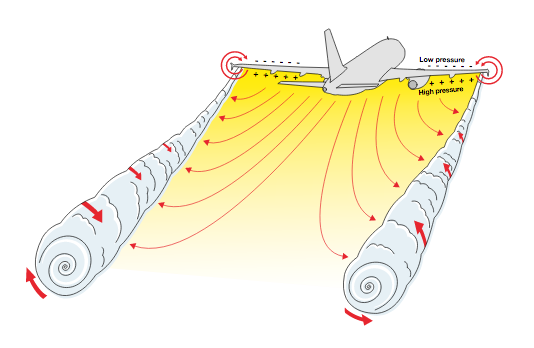
\includegraphics[width=0.8\textwidth]{graphics/WakeVortexPlane.png}
  \caption[RU Logo]{Development of wingtip vortices. Two main vortices form behind the aircraft turning in opposite directions, clockwise behind the left wing (seen from behind) and anti-clockwise behind the right one\cite{magazine_aibus_safety}} \label{fig:vortex_develop}
\end{figure}


\begin{table}
  \centering
  \begin{tabular}{ll}
    $x$& $x^{2}$\\
    1 &1\\
    2 &4\\
    3 &9\\
  \end{tabular}
  \caption{Table of squared numbers}\label{tab:numbers}
\end{table}
%There is an RU logo in Figure~\ref{fig:ru-logo}.
This logo will scale according to the width of the text on the page.
There is a helpful list of squared numbers in Table~\ref{tab:numbers}.

The test text ``Lorem Ipsum''\index{Lorem Ipsum} is from an ancient text from 45 B.C. \cite{cicero46deFinibus, lipsomwebsite}\\
\lipsum[1-5]
\subsection{Subsection}
\lipsum[6-10]
\subsubsection{SubSubsection}
\lipsum[11-15]
%%% Local Variables: 
%%% mode: latex
%%% TeX-master: "DEGREE-NAME-YEAR"
%%% End: 
